\documentclass[10pt,aspectratio=43]{beamer}

\usepackage{graphicx}
\usepackage{tikz}
\usepackage{xcolor}
\usepackage{caption}
\usepackage{subcaption}
\usepackage{bm}
\usetikzlibrary{calc} 
\usepackage{hyperref}
\hypersetup{
    colorlinks=true,
    linkcolor=blue,
    urlcolor=red
}
\usepackage{fontawesome5}
\usepackage{ulem}
\usepackage[dvipsnames]{xcolor}

\usetheme{MyStyle}   % loads beamerthemeMyStyle.sty
\setlength{\columnsep}{0pt}


%%%%%%%%%%%%%%%%%%%%%%%%%%%%%%%%%%%%%%%%%%
%%%%%%%%%%%%%%%%%%%%%%%%%%%%%%%%%%%%%%%%%%
%%%%%%%%%%%%%%%%%%%%%%%%%%%%%%%%%%%%%%%%%%

\title{Time walk study}
\newcommand{\eventname}{ALERT meeting}
\author{Felix Touchte Codjo}
\institute{IJCLab}
\date{\today}


\begin{document}

\begin{frame}[plain] % remove header, footer, barre de navigation
\titlepage
\end{frame}

%\begin{frame}{Outline}
%\tableofcontents
%\end{frame}

%\section{Intro}
\section{Updates}

\begin{frame}{Saturated ADC and time reconstruction}
    \begin{itemize}
        \item Past weeks, I was looking at 4He DVCS in pass 0 data
        \item Remaining issues in the reconstruction has certainly reduced the number of events I was able to see
        \item Particularly, most 4He signals are associated to saturated AHDC pulses
        \item For such signals, the arrival time and the timeOverThreshold can be wrong
    \end{itemize}



    \centering
    \vspace{0.2cm}

    \begin{figure}
        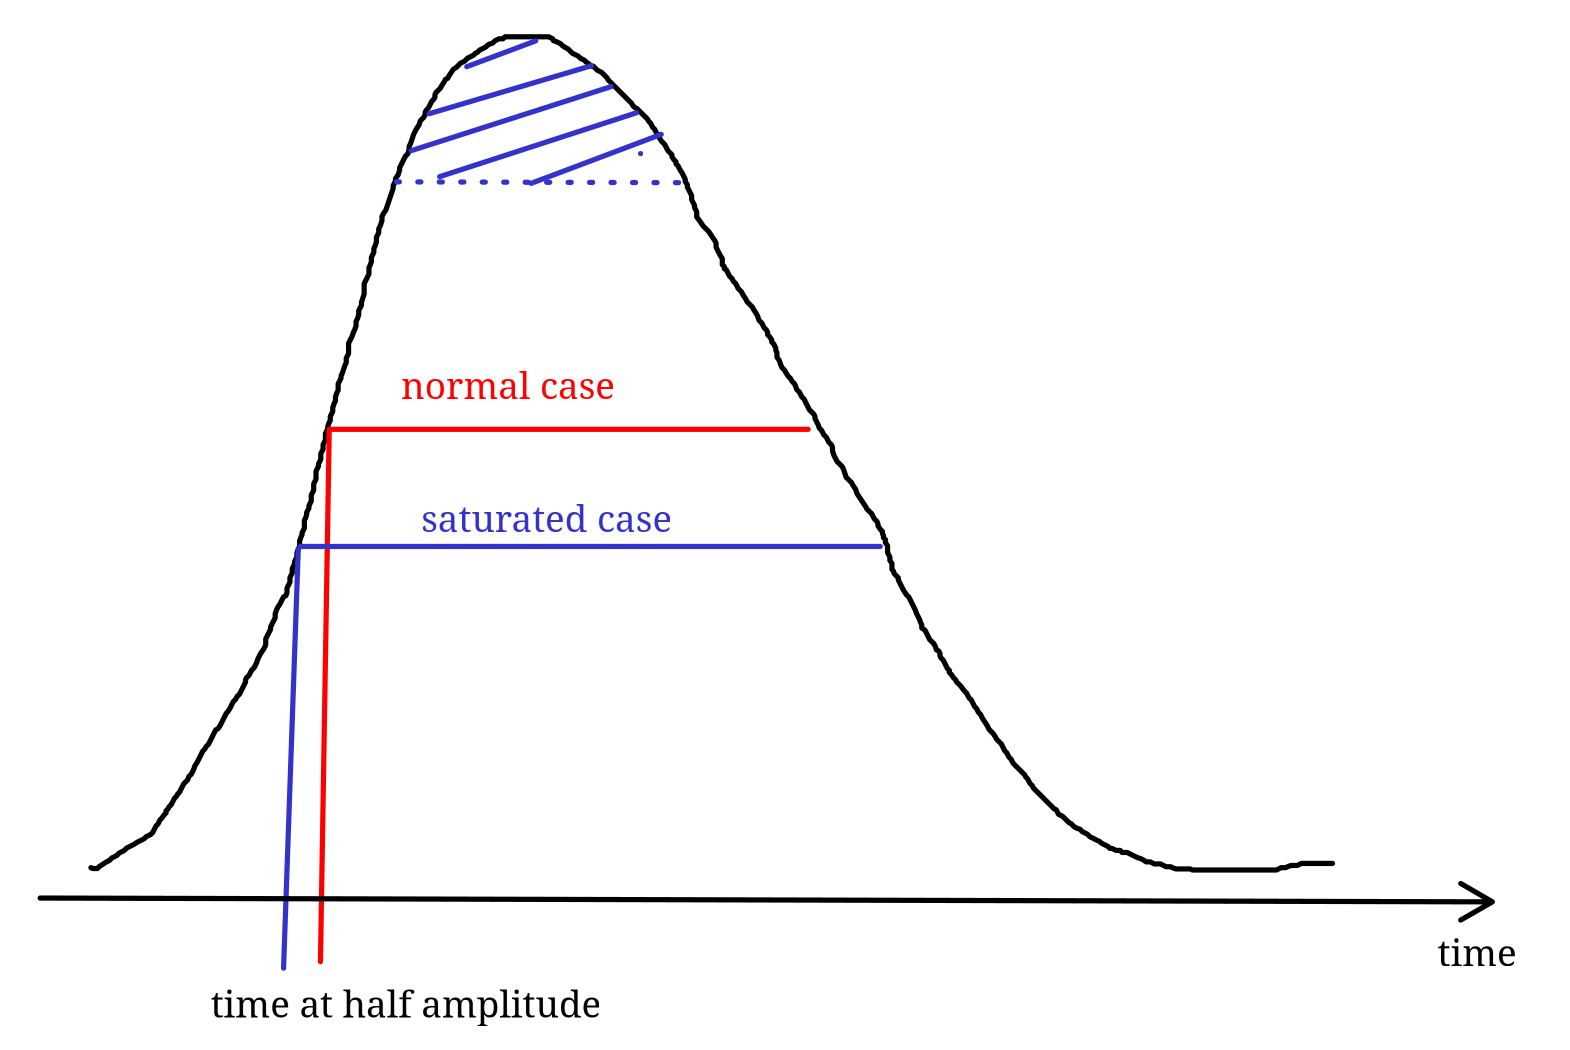
\includegraphics[width=0.6\linewidth]{figures/timewalk.png}
    \end{figure}

\end{frame}

\begin{frame}{Saturated ADC and time reconstruction}
    
    \centering
    % \vspace{0.2cm}

    \begin{minipage}{0.45\linewidth}
        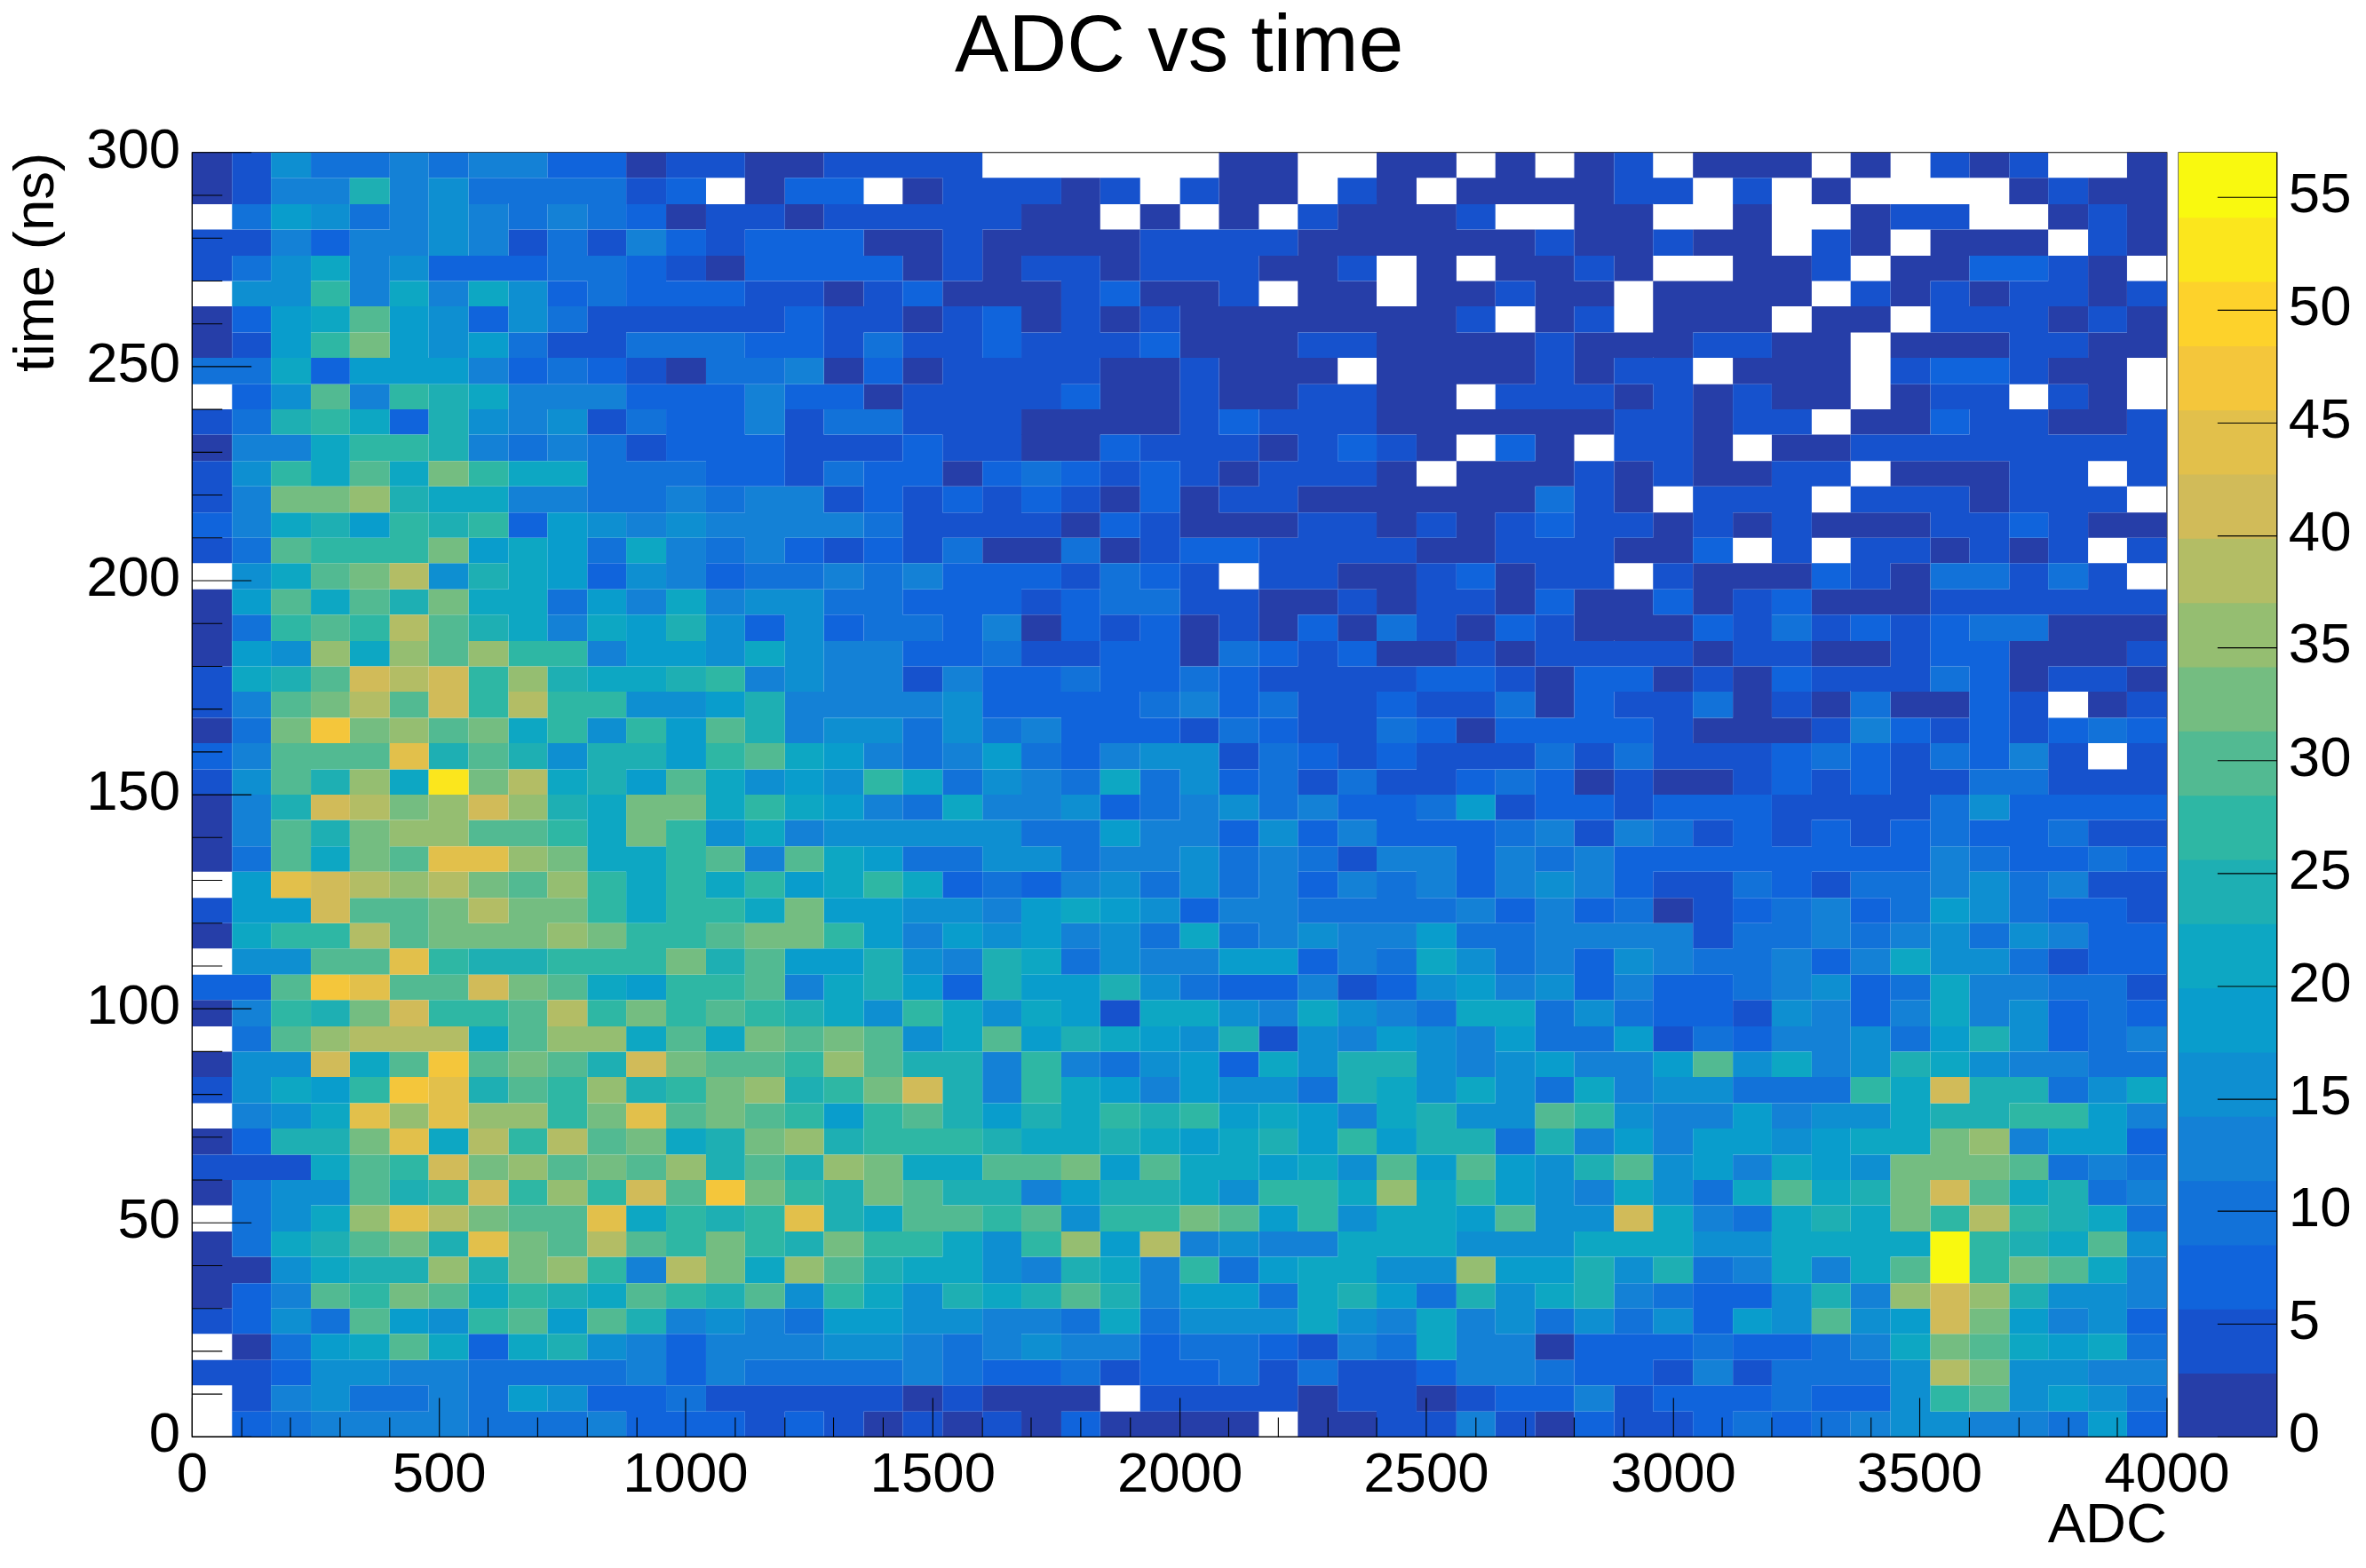
\includegraphics[width=\linewidth]{figures/adc_vs_time.png} \\

        \vspace{0.2cm}

        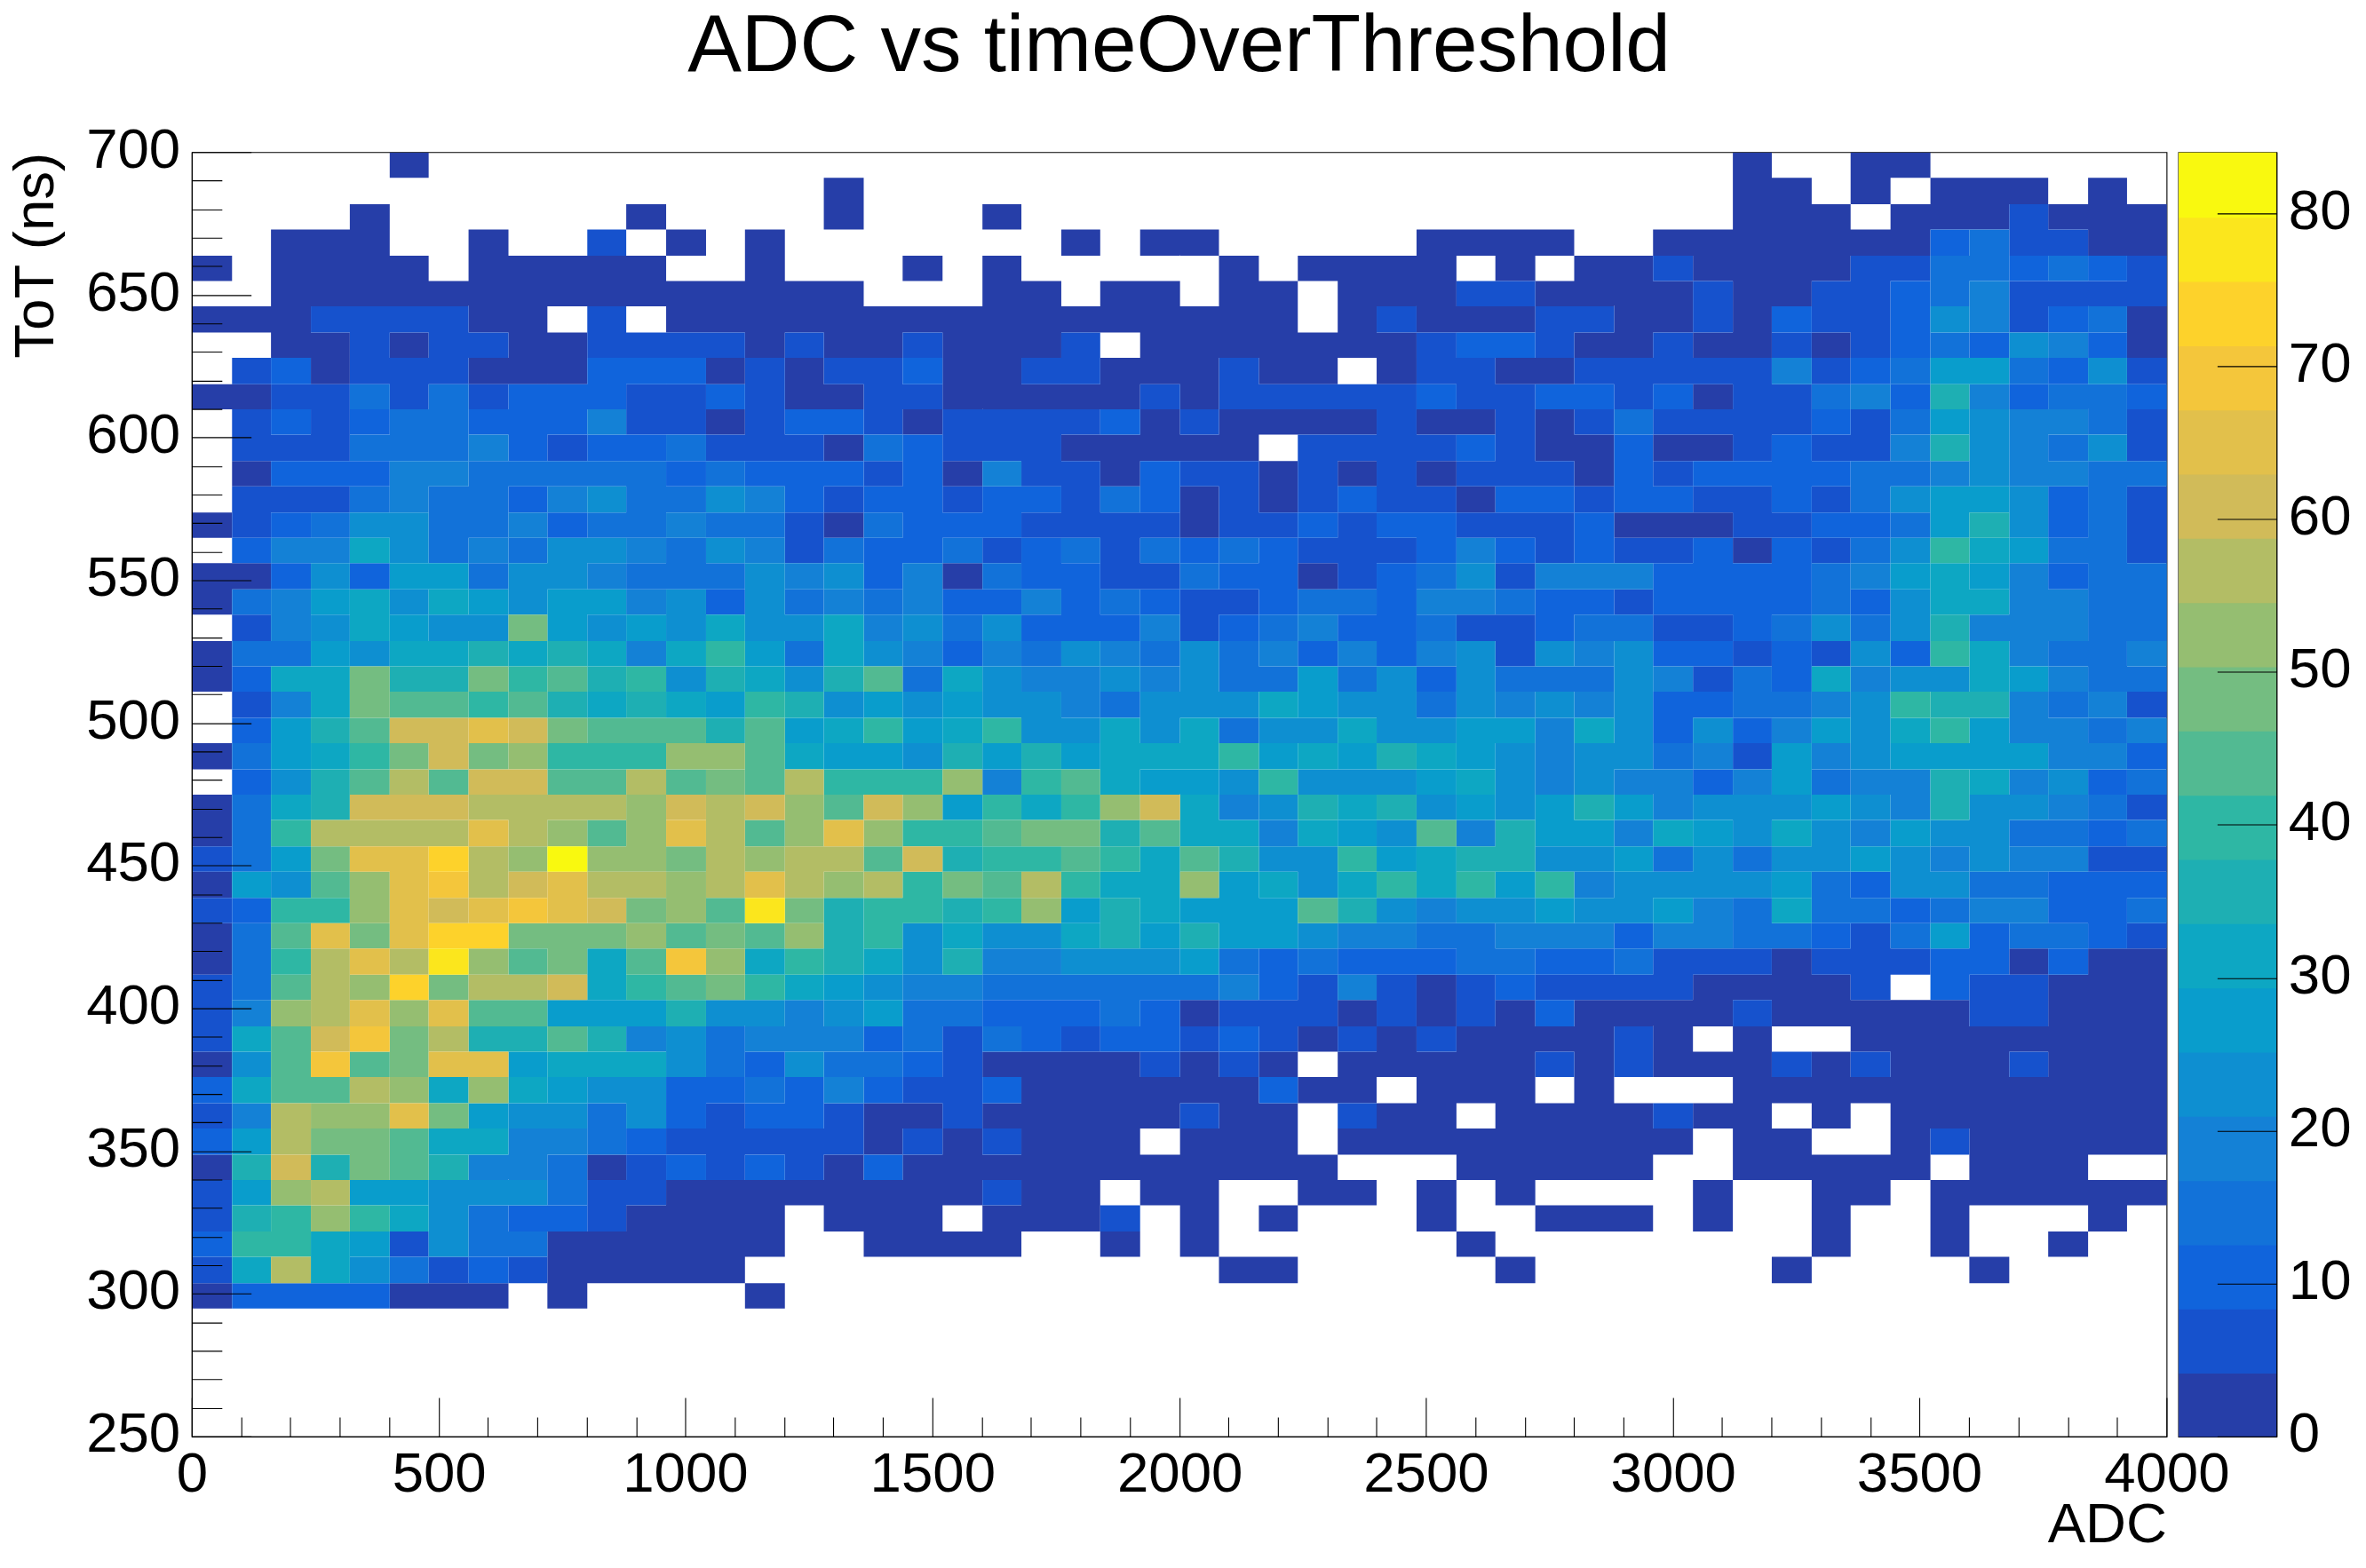
\includegraphics[width=\linewidth]{figures/adc_vs_tot.png}
    \end{minipage}
    \hfill
    \begin{minipage}{0.45\linewidth}
        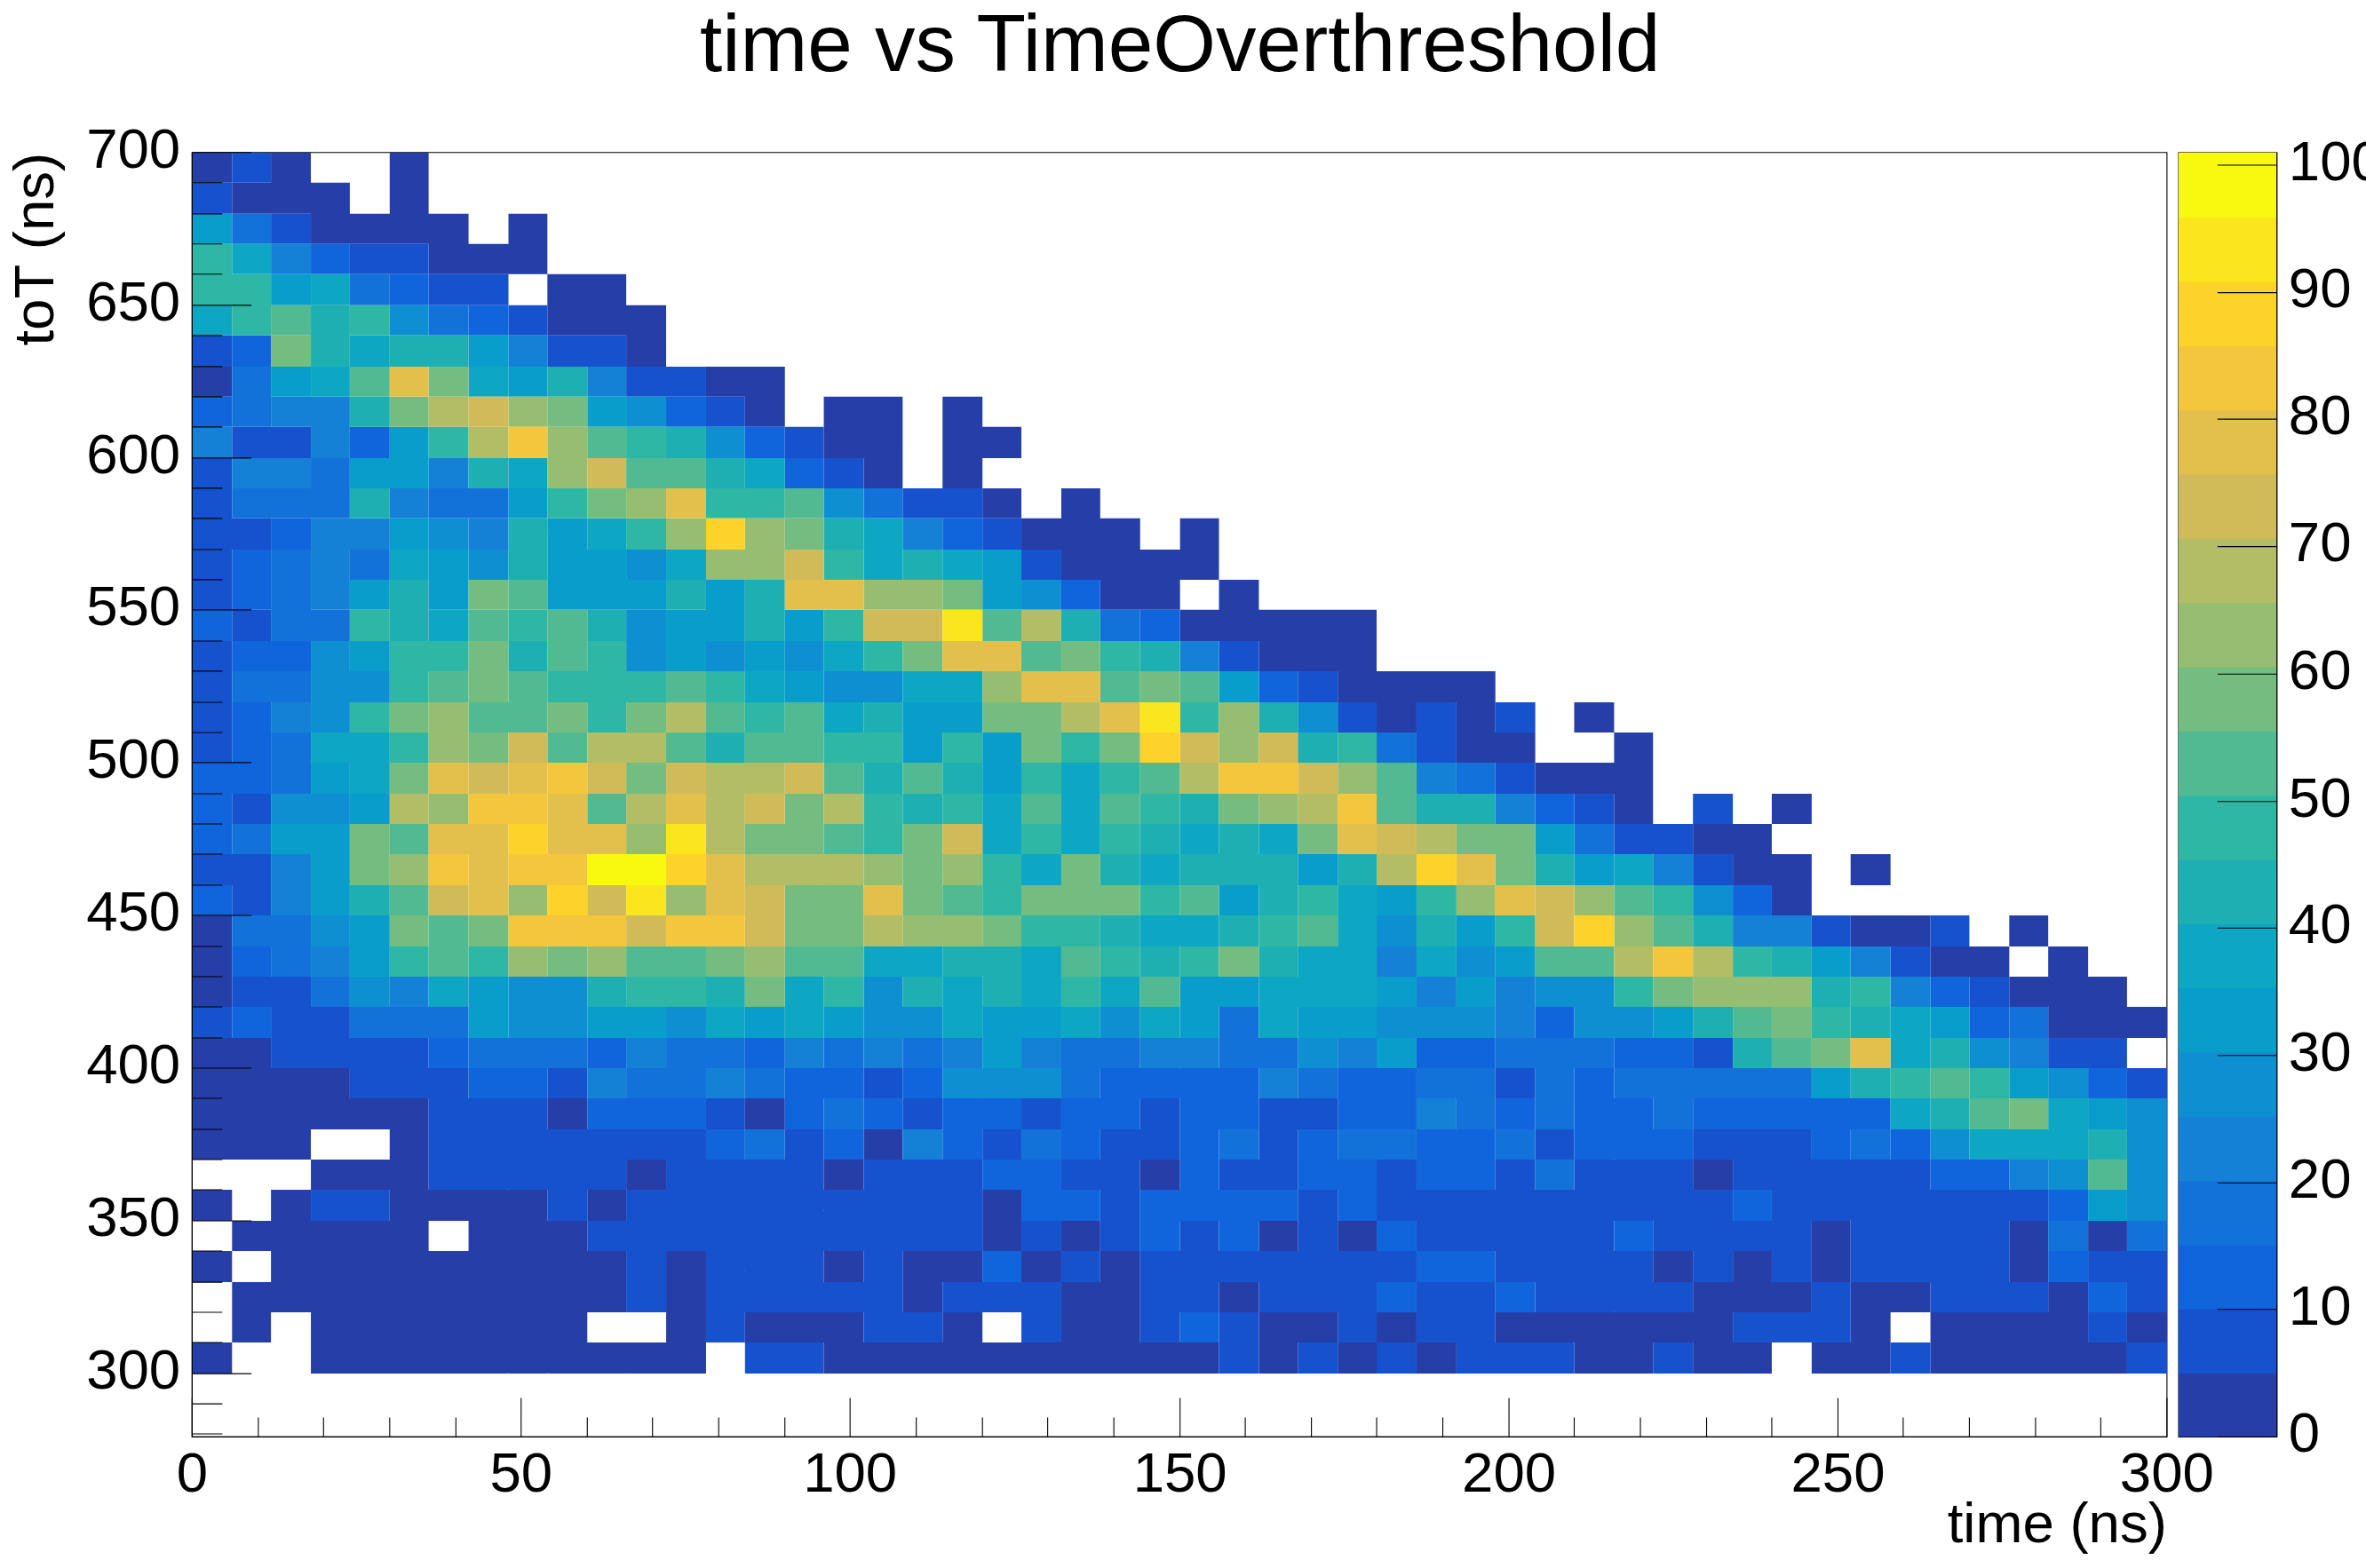
\includegraphics[width=\linewidth]{figures/time_vs_tot.png} \\
        \begin{itemize} \footnotesize
            \item We are particularly interested in early and saturated signals
            \item The plateau in time vs ToT are normal signals
            \item We also have a time walk effect on low ADCs
        \end{itemize}
    \end{minipage}

\end{frame}

\begin{frame}{Strategy}
    \begin{itemize}
        \item measure ToT $\rightarrow$ correct ADC $\rightarrow$ deduce Time
        \item Several approaches
            \begin{itemize}
                \item A fit (as illustrated, need to be improved)
                \item Parametrization by comparing with the residual
                \item Simulation
            \end{itemize}
        \item Validation
            \begin{itemize}
                \item Signals with ADC between 2500-3500
            \end{itemize}
    \end{itemize}



    \centering
    \vspace{0.2cm}

    \begin{figure}
        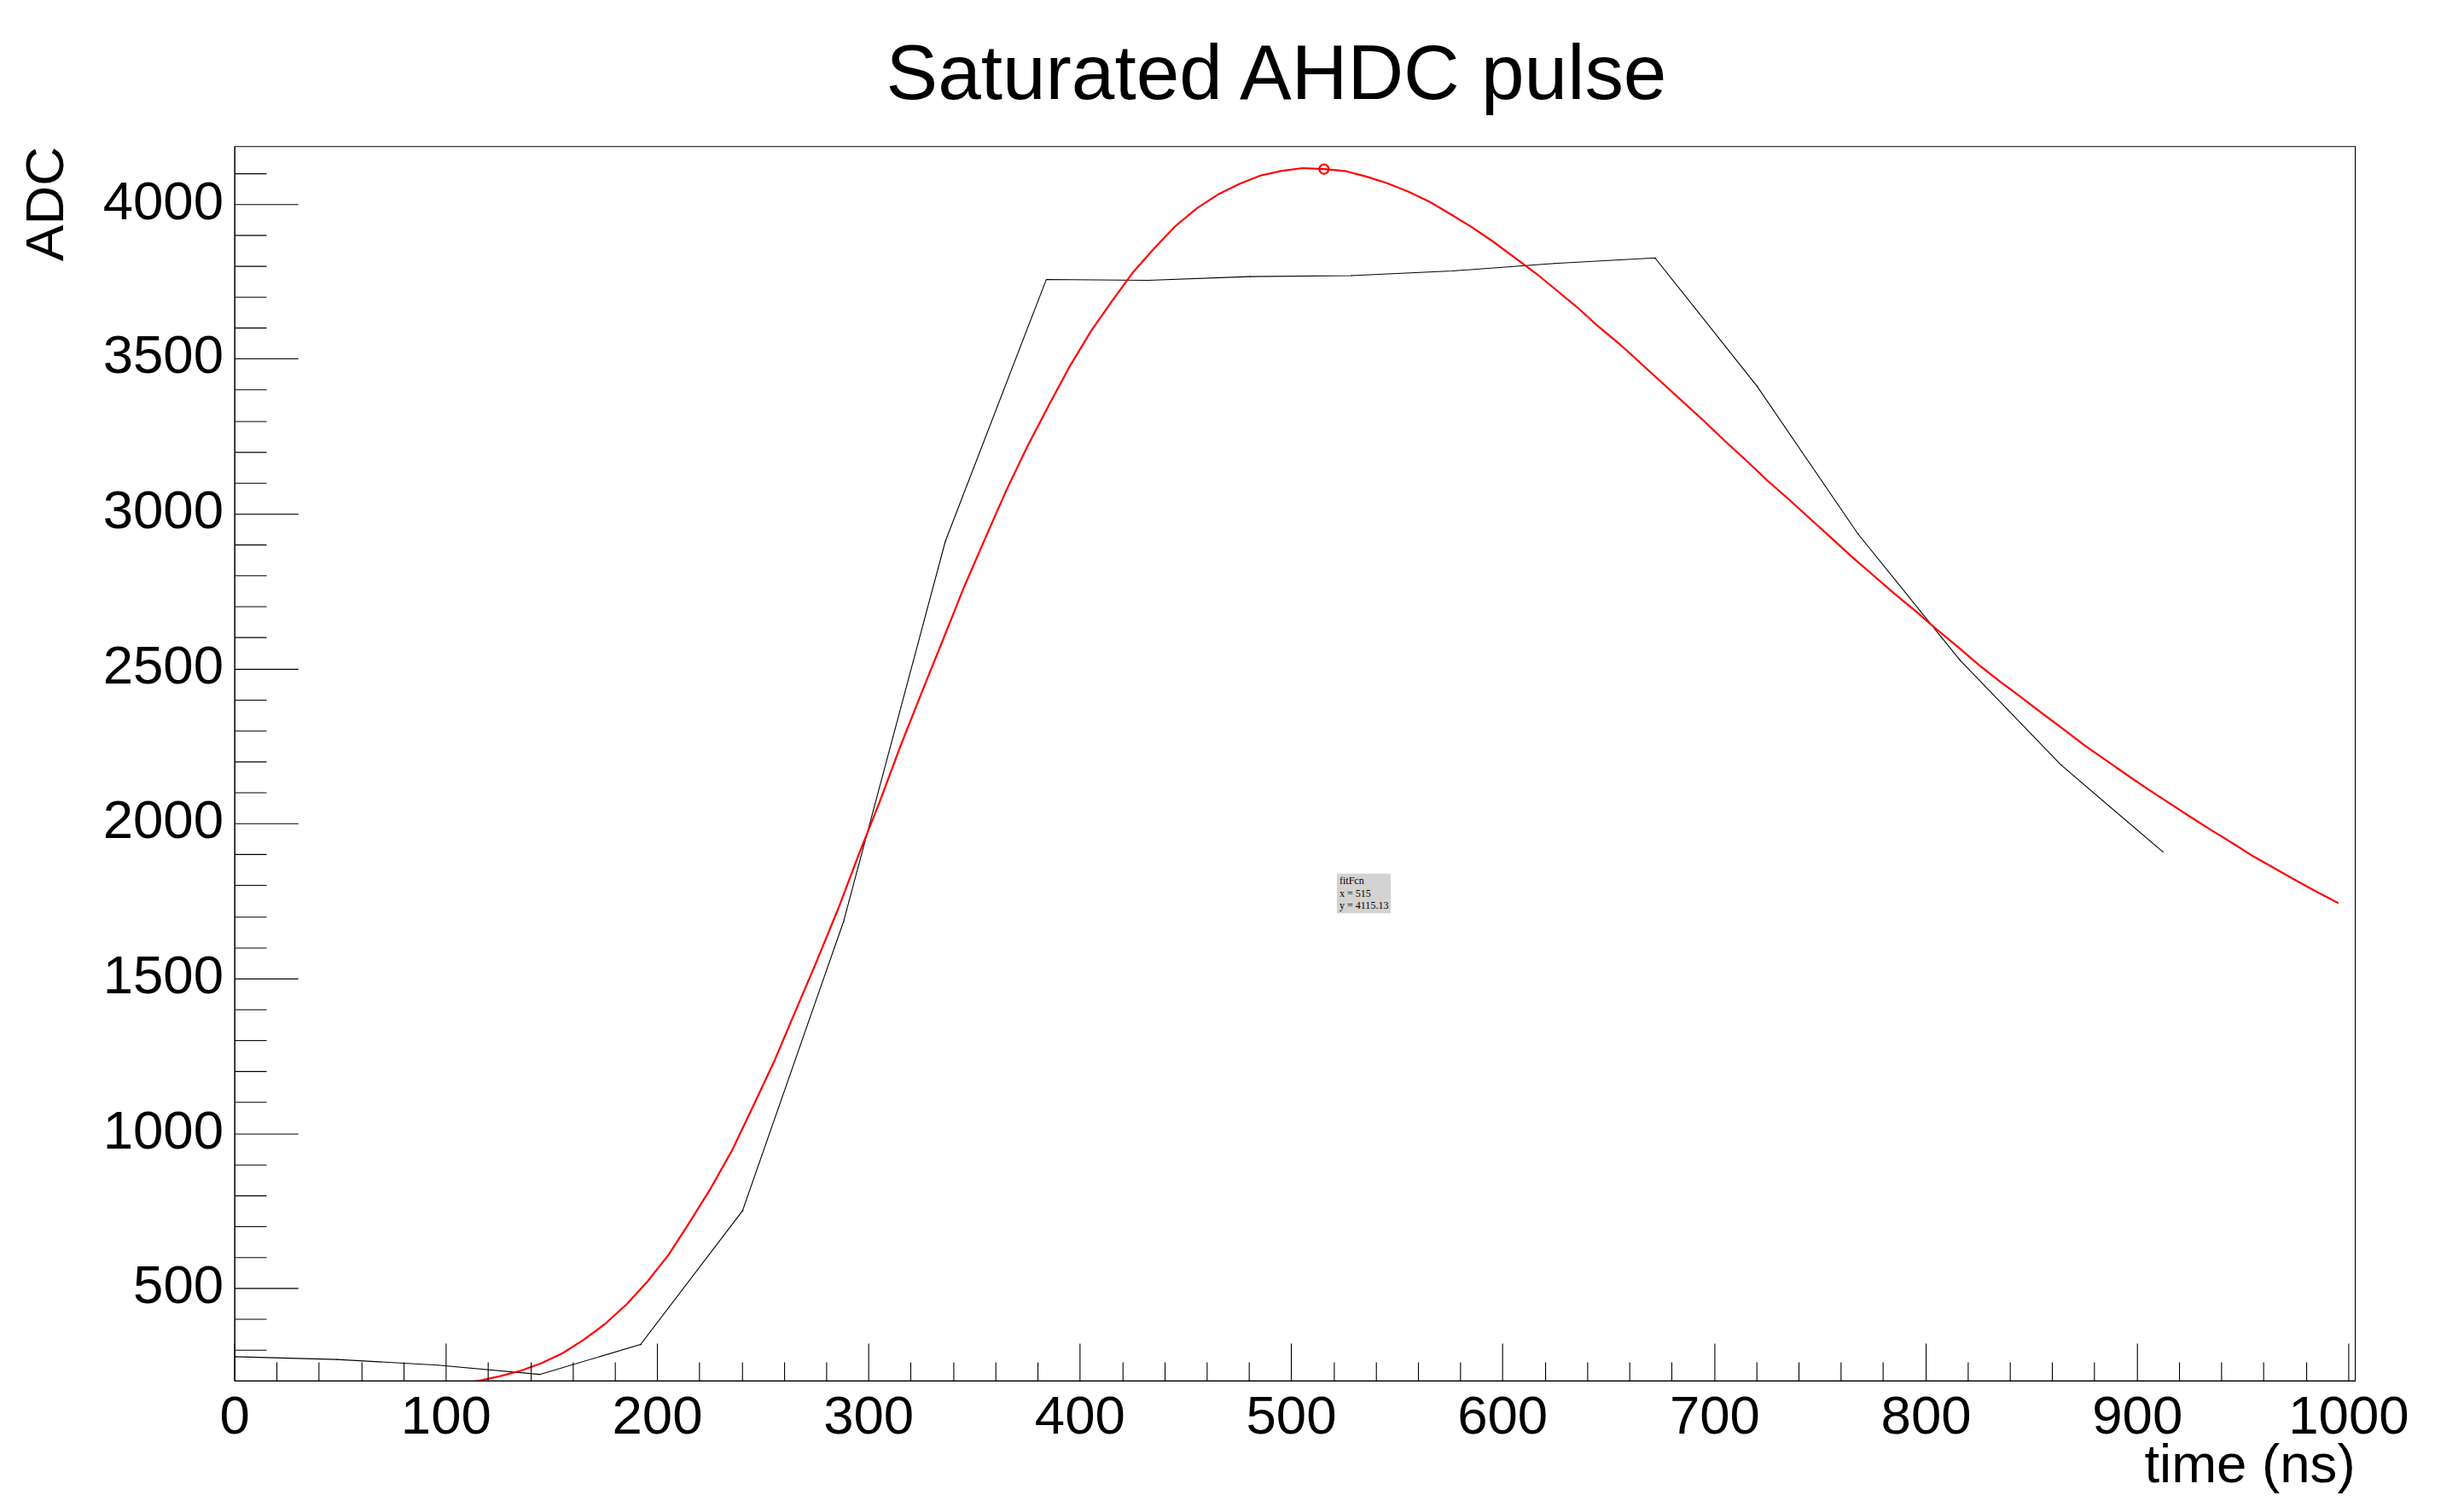
\includegraphics[width=0.6\linewidth]{figures/fitted_pulse.png}
    \end{figure}

\end{frame}










\end{document}


